\begin{frame}[plain,noframenumbering]{}
	\vspace*{2.3cm}
	\begin{center}
		\huge{\colorit{Higher categories}}
	\end{center}
\end{frame}

\begin{frame}[fragile]{Globular sets}
	\pause
	A \colorit{globular set} is $X = \set{X_n}_{n \geq 0}$ together with \defn{source} and \defn{target} maps
	\[
	\begin{tikzcd}[column sep = small]
		X_0 &
		\arrow[l,shift right = 3pt,"\;\so"'] \arrow[l,shift left = 3pt,"\;\ta"] X_1 &
		\arrow[l,shift right = 3pt,"\;\so"'] \arrow[l,shift left = 3pt,"\;\ta"] X_2 &
		\arrow[l,shift right = 3pt,"\;\so"'] \arrow[l,shift left = 3pt,"\;\ta"] \dotsb
	\end{tikzcd}
	\]
	satisfying the \defn{globular identities}: $\so \circ \so = \so \circ \ta$ and $\ta \circ \so = \ta \circ \ta$.
	
	\pause\bigskip
	\colorit{Example} \ $\bG^n$
	
	\begin{center}
		\begin{tikzpicture} [scale = .35]
			\draw node at (-4,0){ };
			\draw node at (4,0){ };
			\draw[fill] (-0.4,0) circle [radius = 3pt];
			
			\draw node at (-0.4,1){$n = 0$} ;
			\draw node at (0,-2.4){} ;
		\end{tikzpicture}
		\begin{tikzpicture} [scale = .35]
			\draw[fill] (-4,0) circle [radius = 3pt];
			\draw[fill] (4,0) circle [radius = 3pt];
			
			\draw [->] (-4,0) [shorten > = 0.2cm, shorten < = 0.2cm,->] to (4,0) ;
			
			\draw node at (0,1){$n = 1$} ;
			\draw node at (-6,-2.4){} ;
		\end{tikzpicture}
		
		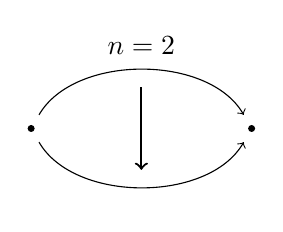
\begin{tikzpicture} [scale = .35]
			\draw[fill] (-4,0) circle [radius = 3pt];
			\draw[fill] (4,0) circle [radius = 3pt];
			
			\draw [->] (-4,0) [shorten > = 0.2cm, shorten < = 0.2cm,->, out = 60,in = 120] to (4,0) ;
			\draw [->] (-4,0) [shorten > = 0.2cm, shorten < = 0.2cm,->, out = -60,in = -120] to (4,0) ;
			
			\draw [->] (0,1.5) [thick] to (0,-1.5) ;
			
			\draw node at (0,3){$n = 2$} ;
		\end{tikzpicture}
		\hspace*{25pt}
		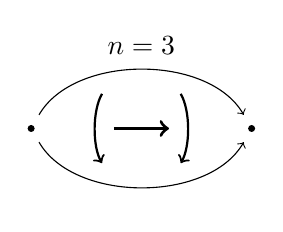
\begin{tikzpicture} [scale = .35]
			\draw[fill] (-4,0) circle [radius = 3pt];
			\draw[fill] (4,0) circle [radius = 3pt];
			
			\draw [->] (-4,0) [shorten > = 0.2cm, shorten < = 0.2cm,->, out = 60,in = 120] to (4,0) ;
			\draw [->] (-4,0) [shorten > = 0.2cm, shorten < = 0.2cm,->, out = -60,in = -120] to (4,0) ;
			
			\draw [->] (-1,2) [thick,shorten > = 0.3cm, shorten < = 0.3cm,->, out = -120,in = 120] to (-1,-2) ;
			\draw [->] (1,2) [thick,shorten > = 0.3cm, shorten < = 0.3cm,->, out = -60,in = 60] to (1,-2) ;
			
			\draw [->] (-1,0) [very thick] to (1,0) ;
			
			\draw node at (0,3){$n = 3$} ;
		\end{tikzpicture}
	\end{center}
\end{frame}

\begin{frame}{Higher categories}
	\pause
	An \colorit{$\omega$-category} is a globular set together with \colorit{compositions} $\circ_k$ and \colorit{identities}, satisfying \textit{associativity}, \textit{unitality}, and \textit{interchange}.
	
	\pause\bigskip
	\colorit{Example}
	Same morphism
	\begin{gather*}
		a \circ_0 (\alpha \circ_{1} \beta) \circ_{0} ( (\gamma \circ_{0} h) \circ_{1} (\delta \circ_{0} h))
		\shortintertext{and}
		(a \circ_{0} \alpha \circ_{0} e \circ_{0} h) \circ_{1} (a \circ_{0} c \circ_{0} \gamma \circ_{0}
		h) \circ_{1} (a \circ_{0} \beta \circ_{0} \delta \circ_{0} h ).
	\end{gather*}
	
	\pause\medskip\colorit{Diagramatically}
	\[
	\begin{tikzcd}[ampersand replacement = \&]
		u \arrow[rr,"a"] \& \& v \arrow[rr,"c"{description},""{auto = false,name = c}]
		\arrow[rr,out = 70,in = 110,"b",""{auto = false,name = b}]
		\arrow[rr,out = -70,in = -110,"d"',""{auto = false,name = p}]
		\arrow[phantom,"\Downarrow \alpha",from = b,to = c]
		\arrow[phantom,"\Downarrow \beta",from = c,to = p]
		\& \& w \arrow[rr,"f"{description},""{auto = false,name = f}] \arrow[rr,out = 70,in = 110,"e",""{auto = false,name = e}]
		\arrow[rr,out = -70,in = -110,"g"',""{auto = false,name = g}] \& \& x \arrow[rr,"h",""{auto = false,name = h}] \& \& y.
		\arrow[phantom,"\Downarrow \gamma",from = e,to = f]
		\arrow[phantom,"\Downarrow \delta",from = f,to = g]
	\end{tikzcd}
	\]
\end{frame}

\begin{frame}[fragile]{Pasting diagrams}
	\pause
	
	Once the images of $a,\dots,h$ and $\alpha,\dots,\delta$ are appropriately assigned, obtain functor from the free $\omega$-category generated by this diagram to any $\omega$-category.
	\[
	\begin{tikzcd}[ampersand replacement = \&]
		u \arrow[rr,"a"] \& \& v \arrow[rr,"c"{description},""{auto = false,name = c}]
		\arrow[rr,out = 70,in = 110,"b",""{auto = false,name = b}]
		\arrow[rr,out = -70,in = -110,"d"',""{auto = false,name = p}]
		\arrow[phantom,"\Downarrow \alpha",from = b,to = c]
		\arrow[phantom,"\Downarrow \beta",from = c,to = p]
		\& \& w \arrow[rr,"f"{description},""{auto = false,name = f}] \arrow[rr,out = 70,in = 110,"e",""{auto = false,name = e}]
		\arrow[rr,out = -70,in = -110,"g"',""{auto = false,name = g}] \& \& x \arrow[rr,"h",""{auto = false,name = h}] \& \& y.
		\arrow[phantom,"\Downarrow \gamma",from = e,to = f]
		\arrow[phantom,"\Downarrow \delta",from = f,to = g]
	\end{tikzcd}
	\]
	
	\pause\medskip Multiple formalization of this idea: Johnson, Street, Steiner, ...
	
	\pause\medskip All rule out directed loops:
	\[
	\begin{tikzcd}[column sep=9pt,row sep=9pt]
		\arrow[d,<-] \arrow[r] \cdot & \arrow[d] \cdot \\
		\arrow[r,,<-] \cdot & \cdot
	\end{tikzcd}
	\]
\end{frame}

\begin{frame}{Simplices as pasting diagrams (Street 1987)}
	\pause
	\begin{center}
		\includegraphics[scale=.28]{aux/street}
	\end{center}
\end{frame}

\begin{frame}{Continued}
	\vspace*{-10pt}
	\begin{center}
		\includegraphics[scale=.25]{aux/street2}
	\end{center}
\end{frame}

\begin{frame}[fragile]{Nerve and realization}
	\pause
	Street's construction defines a functor
	\[
	\simplex \to \Cat_\infty
	\]
	\pause
	and, therefore, a nerve and realization pair
	\[
	\begin{tikzcd}[column sep=small]
		\fR \colon \sSet \rar[shift left=3pt] & \lar[shift left=3pt] \Cat_\infty :\! \rN.
	\end{tikzcd}
	\]
	
	\pause\medskip
	\colorit{Applications}
	
	\bigskip
	The nerve is used to define \colorit{weak} $\infty$-categories (complicial sets).
	
	\bigskip
	The realization is used to compute partition functions of \colorit{local} TQFT's.	
	
	%	\pause\bigskip
	%	\colorit{Disclaimer} This will play no role today.
\end{frame}

\begin{frame}{Kapranov--Voevodsky conjecture}
	\pause
	\colorit{Conjecture (K-V)} Any frame polytope $P$ defines a pasting diagram.
	
	\pause\medskip\colorit{Example}
	\begin{center}
		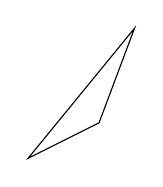
\begin{tikzpicture}[scale=1.5]
			\draw (.3,.7) -- (.9,1) -- (1.2,1.8) -- cycle;
		\end{tikzpicture}
		\begin{tikzpicture}
			\node at (-.5,-.8){+};
			
			\draw[->] (0,-.5) -- (.5,-.5) node[right] {$e_1$};
			\draw[->] (0,-.5) -- (0,-1) node[below] {$-e_2$};
			
			\node at (1.2,-.8){=};
		\end{tikzpicture}
		\begin{tikzpicture}[scale=1.5]
			% Arrowhead in the middle
			\draw[postaction={decorate,decoration={markings,
					mark=at position 0.5 with {\arrow{>}}}}] 
			(.3,.2) -- (.9,.5);
			
			\draw[postaction={decorate,decoration={markings,
					mark=at position 0.5 with {\arrow{>}}}}] 
			(.3,.2) -- (1.2,1.3);
			
			\draw[postaction={decorate,decoration={markings,
					mark=at position 0.5 with {\arrow{>}}}}] 
			(.9,.5) -- (1.2,1.3);
			
			\draw[->, thick] (.76,.64) -- +(-45:.17);
		\end{tikzpicture}
	\end{center}
	
	\pause\bigskip
	We reduced the conjecture to a geometric question.
	
	\medskip
	\colorit{Theorem} $P$ framed defines a pasting diagram iff it has no ``\colorit{cellular loops}''.
	
	\pause\medskip What are cellular loops?
\end{frame}

\begin{frame}{Strings and loops}
	\pause
	A \colorit{$k$-string} in $P$ is a tuple $(F_1,\dots,F_\ell)$ of faces with
	\[
	\ta_k(F_i) \cap \so_k(F_{i+1}) \neq \emptyset.
	\]
	
	\pause
	\colorit{Obs.} This intersection is always a single $k$-face.
	
	\pause\medskip
	\colorit{Example}
	
	\begin{center}
		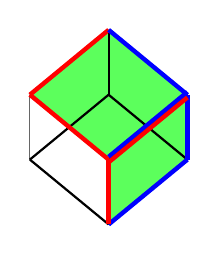
\begin{tikzpicture}
			[
			x = {(0.000000cm, -1.000000cm)},
			y = {(1.000000cm, 0.000000cm)},
			z = {(0.000000cm, 0.000000cm)},
			scale = .700000,
			back/.style = {thin, color = black!60},
			edge/.style = {color = black, thick},
			sourceedge/.style = {color = red, ultra thick},
			targetedge/.style = {color = blue, ultra thick},
			selectededge/.style = {color = green, ultra thick},
			facet/.style = {fill = white,fill opacity = 0.00000},
			targetfacet/.style = {fill = blue!80,fill opacity = 0.800000},
			sourcefacet/.style = {fill = red!80,fill opacity = 0.800000},
			selectedfacet/.style = {fill = green!80,fill opacity = 0.800000},
			vertex/.style = {inner sep = 1pt,circle,draw = black,fill = black,thick},
			targetvertex/.style = {inner sep = 1pt,circle,draw = blue,fill = blue,thick},
			sourcevertex/.style = {inner sep = 1pt,circle,draw = red,fill = red,thick}]
			
			\coordinate (-0.58824, 1.42857, -0.83333) at (-0.58824, 1.42857, -0.83333);
			\coordinate (0.58824, 1.42857, 0.83333) at (0.58824, 1.42857, 0.83333);
			\coordinate (1.76471, 0.00000, 0.00000) at (1.76471, 0.00000, 0.00000);
			\coordinate (0.58824, 0.00000, -1.66667) at (0.58824, 0.00000, -1.66667);
			\coordinate (-0.58824, -1.42857, -0.83333) at (-0.58824, -1.42857, -0.83333);
			\coordinate (-1.76471, 0.00000, 0.00000) at (-1.76471, 0.00000, 0.00000);
			\coordinate (-0.58824, 0.00000, 1.66667) at (-0.58824, 0.00000, 1.66667);
			\coordinate (0.58824, -1.42857, 0.83333) at (0.58824, -1.42857, 0.83333);
			
			\fill[facet] (-0.58824, 0.00000, 1.66667) -- (0.58824, -1.42857, 0.83333) -- (-0.58824, -1.42857, -0.83333) -- (-1.76471, 0.00000, 0.00000) -- cycle {};
			\fill[selectedfacet] (-0.58824, 1.42857, -0.83333) -- (-1.76471, 0.00000, 0.00000) -- (-0.58824, -1.42857, -0.83333) -- (0.58824, 0.00000, -1.66667) -- cycle {};
			\fill[facet] (0.58824, 0.00000, -1.66667) -- (-0.58824, -1.42857, -0.83333) -- (0.58824, -1.42857, 0.83333) -- (1.76471, 0.00000, 0.00000) -- cycle {};
			
			\draw[edge,back] (0.58824, 0.00000, -1.66667) -- (-0.58824, -1.42857, -0.83333);
			\draw[edge,back] (-0.58824, -1.42857, -0.83333) -- (-1.76471, 0.00000, 0.00000);
			\draw[edge,back] (-0.58824, -1.42857, -0.83333) -- (0.58824, -1.42857, 0.83333);
			
			% %% Drawing the facets
			
			\fill[selectedfacet] (0.58824, 0.00000, -1.66667) -- (-0.58824, 1.42857, -0.83333) -- (0.58824, 1.42857, 0.83333) -- (1.76471, 0.00000, 0.00000) -- cycle {};
			\fill[facet] (0.58824, -1.42857, 0.83333) -- (1.76471, 0.00000, 0.00000) -- (0.58824, 1.42857, 0.83333) -- (-0.58824, 0.00000, 1.66667) -- cycle {};
			\fill[facet] (-0.58824, 0.00000, 1.66667) -- (0.58824, 1.42857, 0.83333) -- (-0.58824, 1.42857, -0.83333) -- (-1.76471, 0.00000, 0.00000) -- cycle {};
			
			%% Drawing edges in the front
			
			\draw[edge] (-0.58824, 1.42857, -0.83333) -- (0.58824, 1.42857, 0.83333);
			\draw[edge] (-0.58824, 1.42857, -0.83333) -- (0.58824, 0.00000, -1.66667);
			\draw[edge] (-0.58824, 1.42857, -0.83333) -- (-1.76471, 0.00000, 0.00000);
			\draw[edge] (0.58824, 1.42857, 0.83333) -- (1.76471, 0.00000, 0.00000);
			\draw[edge] (0.58824, 1.42857, 0.83333) -- (-0.58824, 0.00000, 1.66667);
			\draw[edge] (1.76471, 0.00000, 0.00000) -- (0.58824, 0.00000, -1.66667);
			\draw[edge] (1.76471, 0.00000, 0.00000) -- (0.58824, -1.42857, 0.83333);
			\draw[edge] (-1.76471, 0.00000, 0.00000) -- (-0.58824, 0.00000, 1.66667);
			\draw[edge] (-0.58824, 0.00000, 1.66667) -- (0.58824, -1.42857, 0.83333);
			
			\draw[back,sourceedge] (0.58824, 0.00000, -1.66667) -- (-0.58824, -1.42857, -0.83333);
			\draw[back,sourceedge] (-0.58824, -1.42857, -0.83333) -- (-1.76471, 0.00000, 0.00000);
			
			\draw[targetedge] (-0.58824, 1.42857, -0.83333) -- (-1.76471, 0.00000, 0.00000);
			
			\begin{scope}[shift = {(-0.05,-0.0,-0.0)}]
				\draw[targetedge] (-0.58824, 1.42857, -0.83333) -- (0.58824, 0.00000, -1.66667);
			\end{scope}
			
			
			\draw[targetedge] (-0.58824, 1.42857, -0.83333) -- (0.58824, 1.42857, 0.83333);
			\draw[targetedge] (0.58824, 1.42857, 0.83333) -- (1.76471, 0.00000, 0.00000);
			\draw[sourceedge] (1.76471, 0.00000, 0.00000) -- (0.58824, 0.00000, -1.66667);
			\begin{scope}[shift = {(0.05,+0,+0)}]
				\draw[sourceedge] (-0.58824, 1.42857, -0.83333) -- (0.58824, 0.00000, -1.66667);
			\end{scope}
		\end{tikzpicture}
		\qquad\qquad
		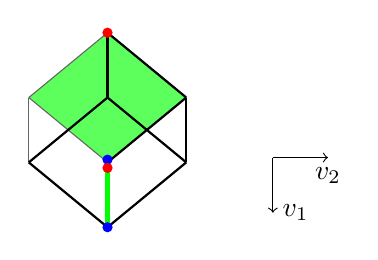
\begin{tikzpicture}
			[
			x = {(0.000000cm, -1.000000cm)},
			y = {(1.000000cm, 0.000000cm)},
			z = {(0.000000cm, 0.000000cm)},
			scale = .700000,
			back/.style = {thin, color = black!60},
			edge/.style = {color = black, thick},
			sourceedge/.style = {color = red, ultra thick},
			targetedge/.style = {color = blue, ultra thick},
			selectededge/.style = {color = green, ultra thick},
			facet/.style = {fill = white,fill opacity = 0.00000},
			targetfacet/.style = {fill = blue!80,fill opacity = 0.800000},
			sourcefacet/.style = {fill = red!80,fill opacity = 0.800000},
			selectedfacet/.style = {fill = green!80,fill opacity = 0.800000},
			vertex/.style = {inner sep = 1pt,circle,draw = black,fill = black,thick},
			targetvertex/.style = {inner sep = 1pt,circle,draw = blue,fill = blue,thick},
			sourcevertex/.style = {inner sep = 1pt,circle,draw = red,fill = red,thick}]
			
			\coordinate (-0.58824, 1.42857, -0.83333) at (-0.58824, 1.42857, -0.83333);
			\coordinate (0.58824, 1.42857, 0.83333) at (0.58824, 1.42857, 0.83333);
			\coordinate (1.76471, 0.00000, 0.00000) at (1.76471, 0.00000, 0.00000);
			\coordinate (0.58824, 0.00000, -1.66667) at (0.58824, 0.00000, -1.66667);
			\coordinate (-0.58824, -1.42857, -0.83333) at (-0.58824, -1.42857, -0.83333);
			\coordinate (-1.76471, 0.00000, 0.00000) at (-1.76471, 0.00000, 0.00000);
			\coordinate (-0.58824, 0.00000, 1.66667) at (-0.58824, 0.00000, 1.66667);
			\coordinate (0.58824, -1.42857, 0.83333) at (0.58824, -1.42857, 0.83333);
			
			\fill[facet] (-0.58824, 0.00000, 1.66667) -- (0.58824, -1.42857, 0.83333) -- (-0.58824, -1.42857, -0.83333) -- (-1.76471, 0.00000, 0.00000) -- cycle {};
			\fill[selectedfacet] (-0.58824, 1.42857, -0.83333) -- (-1.76471, 0.00000, 0.00000) -- (-0.58824, -1.42857, -0.83333) -- (0.58824, 0.00000, -1.66667) -- cycle {};
			\fill[facet] (0.58824, 0.00000, -1.66667) -- (-0.58824, -1.42857, -0.83333) -- (0.58824, -1.42857, 0.83333) -- (1.76471, 0.00000, 0.00000) -- cycle {};
			
			
			\draw[edge,back] (0.58824, 0.00000, -1.66667) -- (-0.58824, -1.42857, -0.83333);
			\draw[edge,back] (-0.58824, -1.42857, -0.83333) -- (-1.76471, 0.00000, 0.00000);
			\draw[edge,back] (-0.58824, -1.42857, -0.83333) -- (0.58824, -1.42857, 0.83333);
			
			%% Drawing the facets
			
			\fill[facet] (0.58824, 0.00000, -1.66667) -- (-0.58824, 1.42857, -0.83333) -- (0.58824, 1.42857, 0.83333) -- (1.76471, 0.00000, 0.00000) -- cycle {};
			\fill[facet] (0.58824, -1.42857, 0.83333) -- (1.76471, 0.00000, 0.00000) -- (0.58824, 1.42857, 0.83333) -- (-0.58824, 0.00000, 1.66667) -- cycle {};
			\fill[facet] (-0.58824, 0.00000, 1.66667) -- (0.58824, 1.42857, 0.83333) -- (-0.58824, 1.42857, -0.83333) -- (-1.76471, 0.00000, 0.00000) -- cycle {};
			
			%% Drawing edges in the front
			
			\draw[edge] (-0.58824, 1.42857, -0.83333) -- (0.58824, 1.42857, 0.83333);
			\draw[edge] (-0.58824, 1.42857, -0.83333) -- (0.58824, 0.00000, -1.66667);
			\draw[edge] (-0.58824, 1.42857, -0.83333) -- (-1.76471, 0.00000, 0.00000);
			\draw[edge] (0.58824, 1.42857, 0.83333) -- (1.76471, 0.00000, 0.00000);
			\draw[edge] (0.58824, 1.42857, 0.83333) -- (-0.58824, 0.00000, 1.66667);
			\draw[selectededge] (1.76471, 0.00000, 0.00000) -- (0.58824, 0.00000, -1.66667);
			\draw[edge] (1.76471, 0.00000, 0.00000) -- (0.58824, -1.42857, 0.83333);
			\draw[edge] (-1.76471, 0.00000, 0.00000) -- (-0.58824, 0.00000, 1.66667);
			\draw[edge] (-0.58824, 0.00000, 1.66667) -- (0.58824, -1.42857, 0.83333);
			
			% %% Drawing the vertices in the front
			
			\node[targetvertex] at (1.76471, 0.00000, 0.00000)  {};
			
			\node[sourcevertex] at (-1.76471, 0.00000, 0.00000)  {};
			
			\begin{scope}[shift = {(-0.05,-0.0,-0.0)}]
				\node[targetvertex] at (0.58824, 0.00000, -1.66667)  {};
			\end{scope}
			
			\begin{scope}[shift = {(0.1,+0,+0)}]
				\node[sourcevertex] at (0.58824, 0.00000, -1.66667)  {};
			\end{scope}
			%%
			%%
			\begin{scope}[shift = {(.5,3,0)}]
				
				%axes
				\draw[->] (0, 0,0) -- (1, 0,0) node[anchor = west]{$v_1$};
				\draw[->] (0, 0,0) -- (0, 1,0) node[anchor = north]{$v_2$};
				% 		\draw[->] (0, 0,0) -- (0, 0, 1) node[anchor = west]{$v_3$};
			\end{scope}
		\end{tikzpicture}
	\end{center}
	
	\pause\medskip
	We say it is a \colorit{$k$-loop} if $F_i = F_j$ for some $i \neq j$.
	
\end{frame}

\begin{frame}{A 1-loop of 2-faces in the 5-simplex}
	\pause
	Consider $p_1,\dots,p_6 \in \R^5$
	\[
	\begin{pmatrix}
		-3 \\
		-1 \\
		-1 \\
		0 \\
		1
	\end{pmatrix}
	\begin{pmatrix}
		-2 \\
		1 \\
		1 \\
		0 \\
		1
	\end{pmatrix}
	\begin{pmatrix}
		-1 \\
		0 \\
		0 \\
		1 \\
		1
	\end{pmatrix}
	\begin{pmatrix}
		1 \\
		0 \\
		0 \\
		1 \\
		0
	\end{pmatrix}
	\begin{pmatrix}
		2 \\
		1 \\
		-1 \\
		0 \\
		0
	\end{pmatrix}
	\begin{pmatrix}
		3 \\
		-1 \\
		1 \\
		0 \\
		0
	\end{pmatrix}
	\]
	They form a $5$-simplex $P$ and the canonical frame is $P$-admissible.
	
	\pause\medskip
	
	\resizebox{\linewidth}{!}{
		\begin{tikzpicture}[auto, node distance=2cm, >=latex',
			point/.style = {draw, circle, fill = black, inner sep = 1pt}]
			
			\coordinate (a) at (-3,-1);
			\coordinate (b) at (-2,1);
			\coordinate (c) at (-1,0);
			\coordinate (d) at (1,0);
			\coordinate (e) at (2,1);
			\coordinate (f) at (3,-1);
			
			\draw[thick] (c) -- (f) -- (b) -- (d);
			\draw[line width = 3pt,white] (d) -- (a) -- (e) -- (c);
			\draw[thick] (d) -- (a) -- (e) -- (c);
			\draw[thick] (a) -- (b) -- (c) -- (a);
			\draw[thick] (d) -- (e) -- (f) -- (d);
			
			\foreach \i/\l in {a/p_1,b/p_2,c/p_3,d/p_4,e/p_5,f/p_6}
			{
				\node[point,label={above:$\l$}] at (\i) {};
			}
			
			\draw[->] (4,0)-- (4,1);
			\draw[->] (4,0)-- (5,0);
			\node[] at (5.5, 0) {$e_1$};
			\node[] at (4.5, 1) {$e_2$};
	\end{tikzpicture}}
\end{frame}

\begin{frame}{A weaker version}
	\pause
	\colorit{Question} Does every polytope admits a loop-free frame?
	
	\pause\bigskip
	\colorit{Theorem} There is a $4$-polytope for which every admissible frame induces a cellular loop.
\end{frame}

\begin{frame}{The cyclic $n$-simplex}
	\pause
	$\gsimplex_n$ is the convex closure of
	\[
	\set[\big]{(t,t^2,\dots,t^n) \mid t \in \{0,\dots,n-1\}}.
	\]
	
	\begin{minipage}{.35\textwidth}
		\colorit{Example}\par
		\begin{center}
			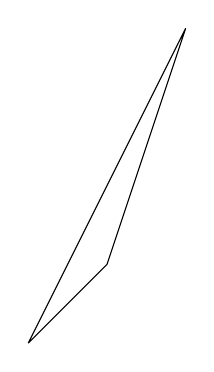
\begin{tikzpicture}
				\draw (0,0)--(1,1)--(2,4)--(0,0);
			\end{tikzpicture}
		\end{center}
	\end{minipage}
	\begin{minipage}{.6\textwidth}
		\pause
		\colorit{Theorem}
		The frame
		\[
		\{e_1,-e_2,e_3,-e_4,\dots\}
		\]
		is $\gsimplex_n$-admissible and loop-free.
		Furthermore, it recovers Street's pasting diagrams.
	\end{minipage}
\end{frame}

\begin{frame}{Gaussian simplices}
	\pause
	\colorit{Question}
	How special is the cyclic embedding?
	
	\pause\bigskip
	A \colorit{Gaussian $n$-simplex} is the convex hull of $n+1$ independent random points in~$\R^n$ each chosen according to a $n$-dim'l std. normal distribution.
	
	\pause\bigskip
	\colorit{Theorem} The probability that a canonically framed Gaussian $n$-simplex has a loop tends to~$1$ as~$n$ tends to~$\infty$.
\end{frame}